\section{Motivational Example}
\label{sec:example}

In this section we present two simple examples that illustrate the
complementary strengths and weaknesses of learning and control.  We
run our examples on mobile development boards featuring Samsung's
Exynos 5 Octa with an ARM big.LITTLE architecture that has four
energy-efficient LITTLE cores and four high-performance big cores.
Each core cluster can be set to different clock speed, leading to a
large configuration space for assigning resources to multi-threaded
applications.

Each configuration (assignment of cores and clockspeeds) has different
performance, and this performance will be application dependent.
\figref{contour} shows how performance varies as a function of both
resource usage and application.  The figures show cores on the x-axis
and clockspeed on the y-axis, with performance shown as intensity --
darker colors representing higher performance. The presence of local
minima and maxima mean that simple gradient ascent/descent methods are
not suitable to navigating these tradeoff spaces.
\figref{fig:contour} shows that the performance plot for the
applications \texttt{kmeans} and \texttt{lavamd} against the
clockspeed and cores is non-convex and contains at least 2 local
minima corresponding to big and LITTLE cores.  In addition,
\texttt{lavamd} has other local minima and has a significantly more
complicated tradeoff space than \texttt{kmeans}. 


\begin{figure}
\centering
%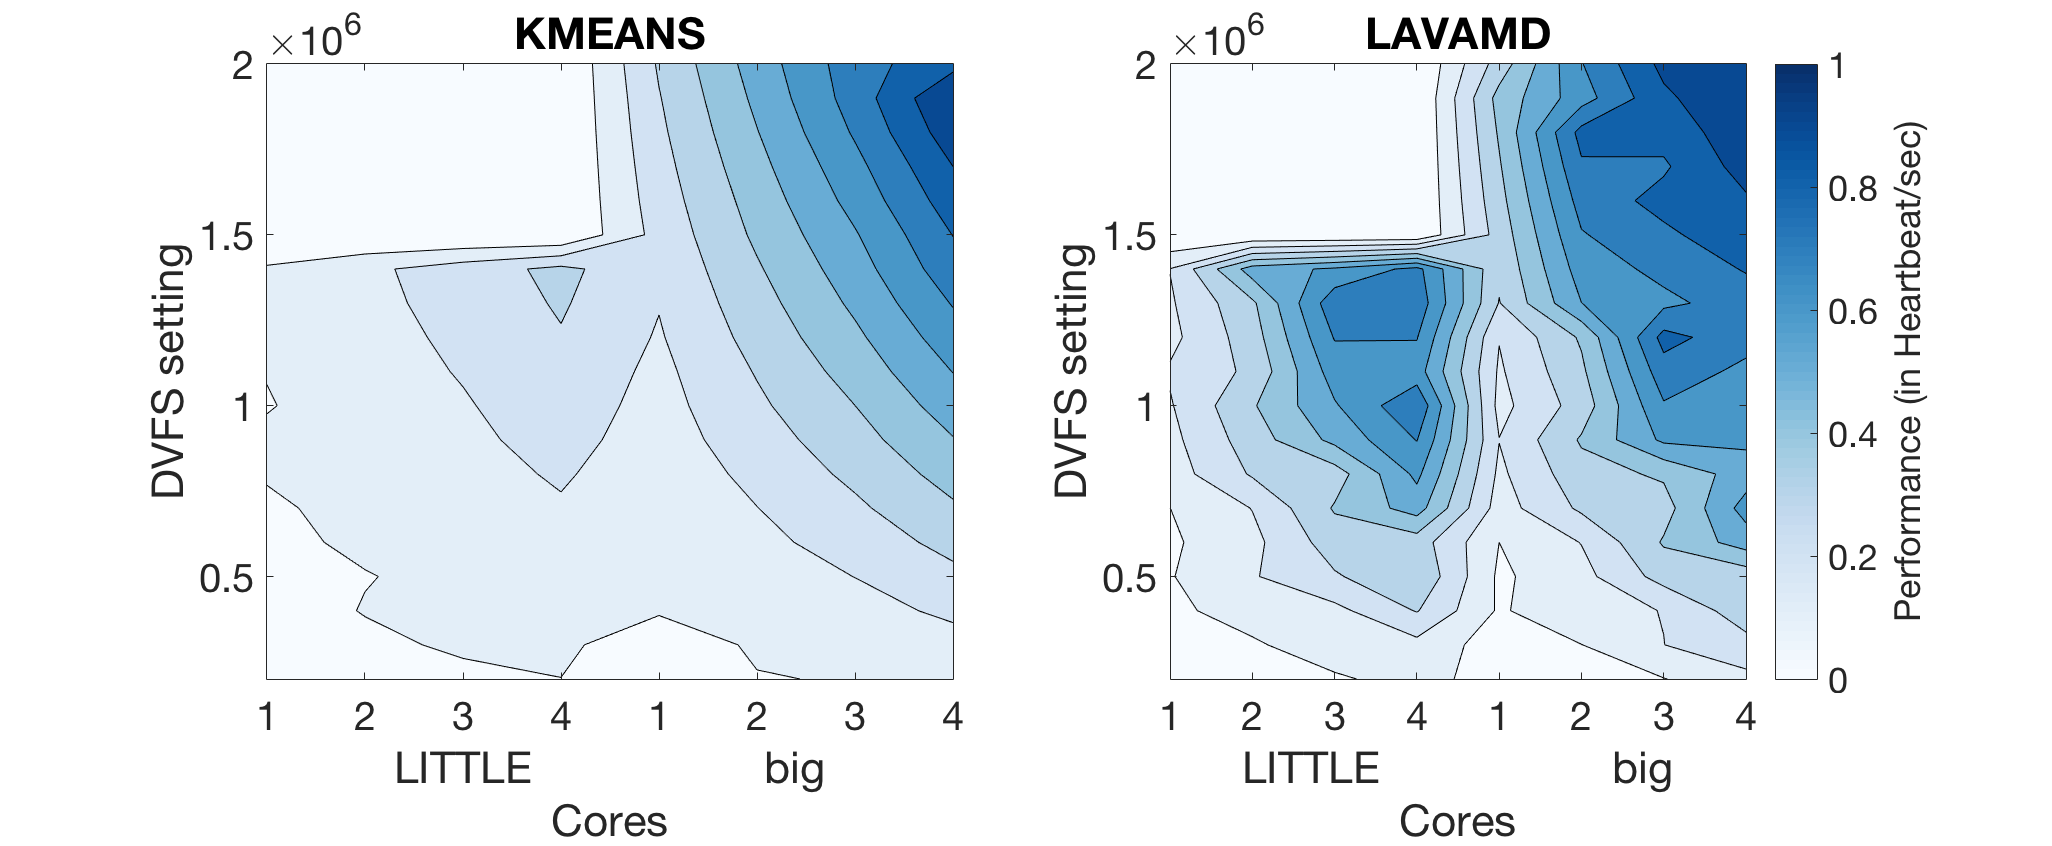
\includegraphics[width=\paperwidth,scale=0.5]{figures/performance-contour2.png}
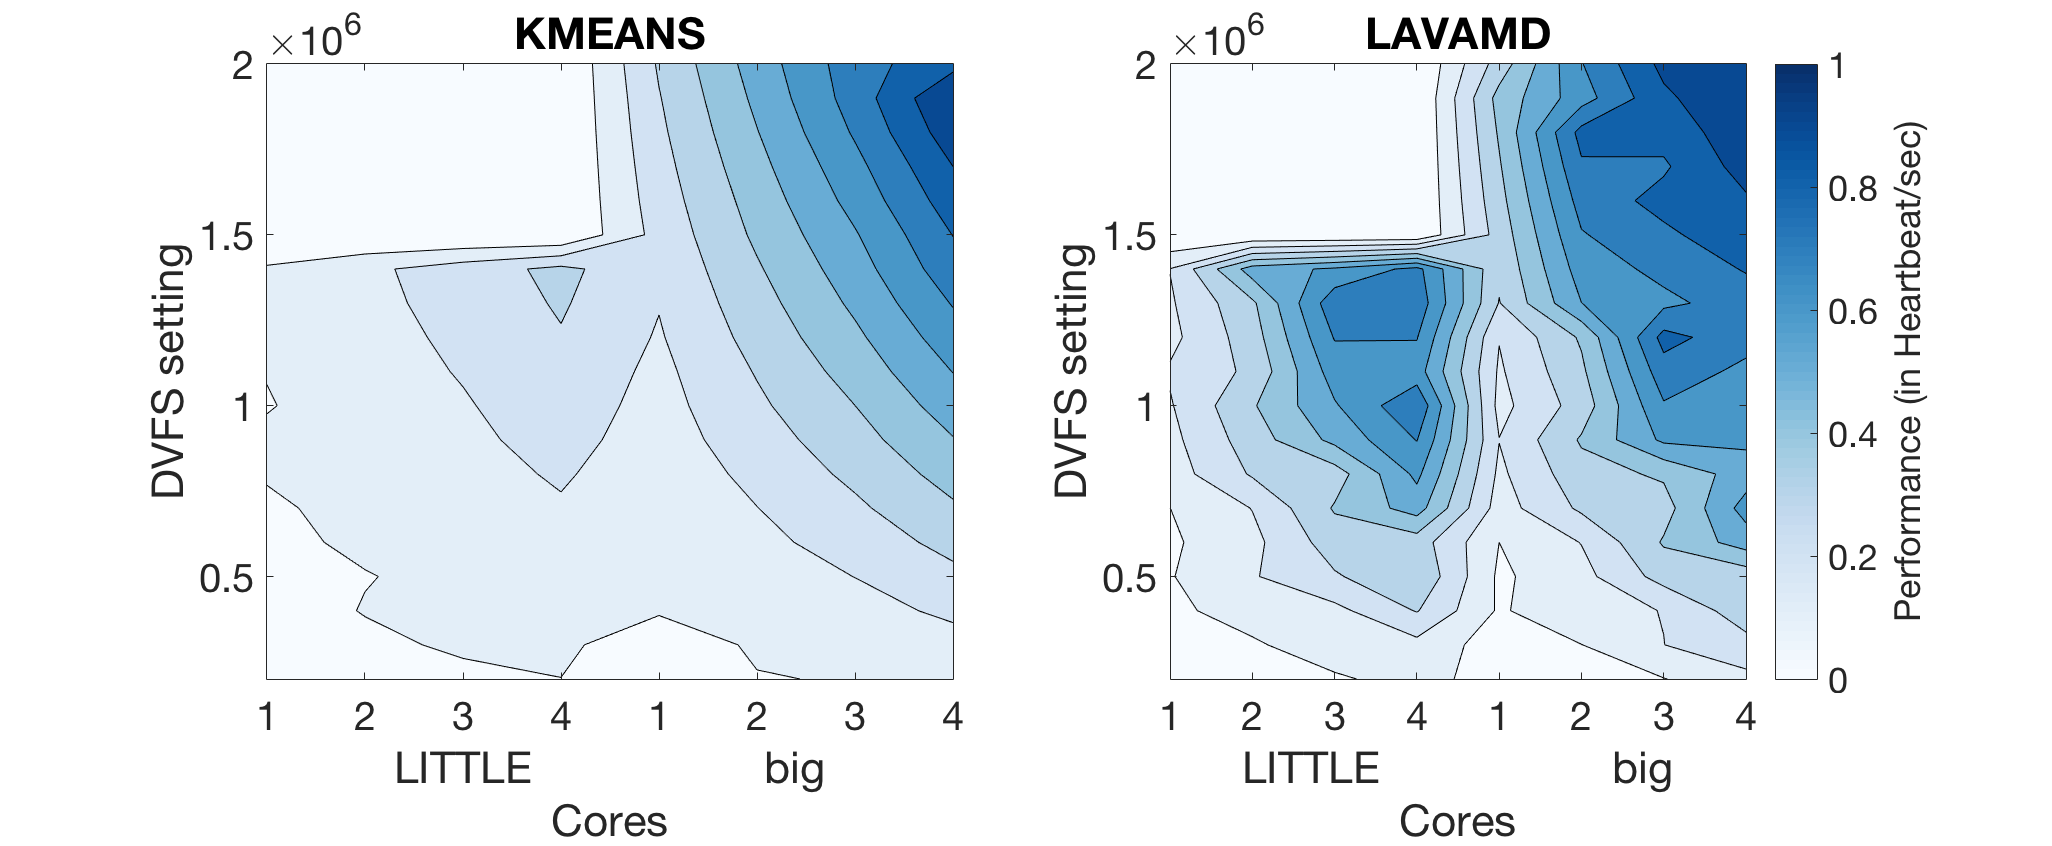
\includegraphics[width=\columnwidth]{figures/performance-contour2.png}
%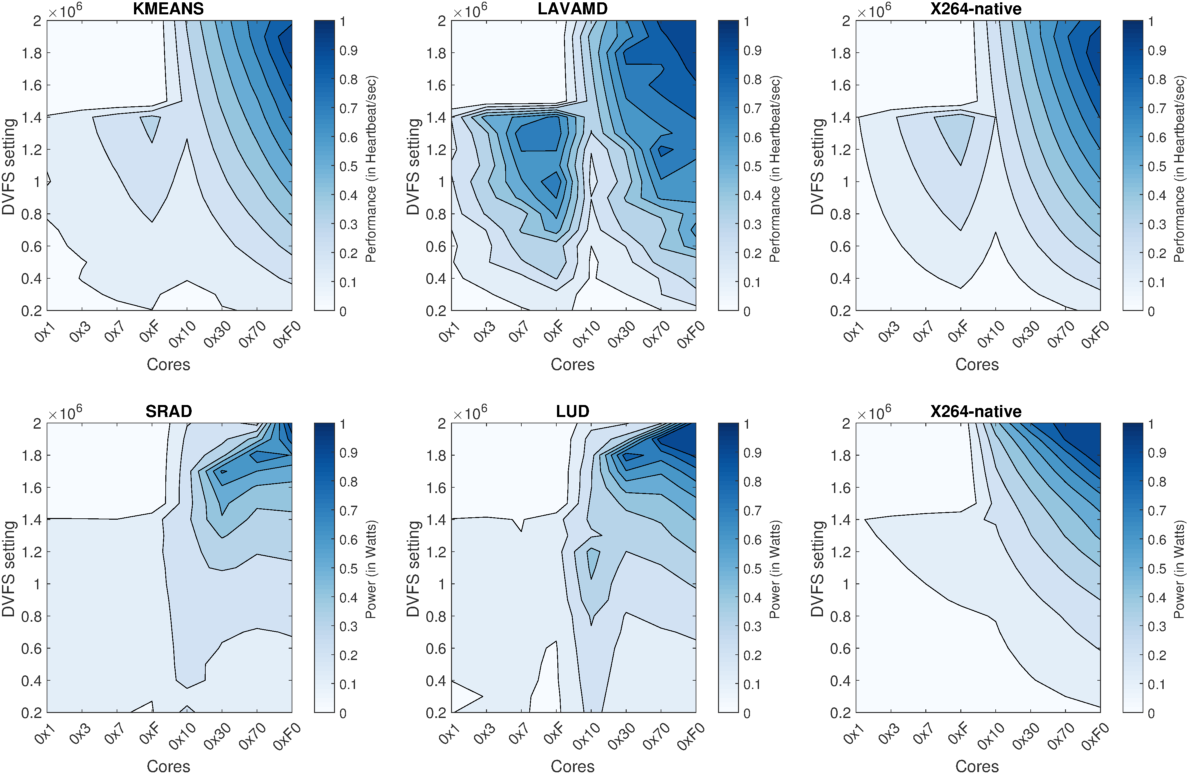
\includegraphics[scale=0.4]{figures/sample-contour3.png}
\caption{Contour plots showing performance as a function of core
  number, type, and speed.}
  \label{fig:contour}
\end{figure}


\subsection{Complexity}
A number of machine learning approaches have been proposed to estimate
application performance in a variety of scenarios
\cite{reddiHPCA2013,LeeBrooks2006,CPR,ParallelismDial,Flicker,LeeBrooks,Koala}.
Machine learning is well suited to building models of complicated
systems like those shown in \figref{contour}.  In this example we
consider LEO, a hierarchical Bayesian model that estimates application
performance as a function of its resource usage \cite{LEO}. We compare
LEO to POET, a control system designed to adjust resource usage to
meet application performance requirements with minimal energy
\cite{POET}.

To demonstrate how well suited learning is to managing complexity, we
consider meeting a performance requirement for \texttt{lavamd}, the
application with the more complicated configuration space.  We launch
the application with a soft performance constraint and both LEO and
POET adjust resource usage to meet that requirement with minimal
resource usage.  LEO works by estimating the performance ad power of
all configurations and then using the lowest power configuration that
meets the goal.  POET works by constantly measuring performance and
adjusting resource usage to see that goals are met.  While many
controllers use linear models, POET uses a convex model and handles
some non-linearities; however, it is sensitive to local maxima.

\begin{figure}[t]
  \begin{tikzpicture}
\begin{centering}

\definecolor{s1}{RGB}{228, 26, 28}
\definecolor{s2}{RGB}{55, 126, 184}
\definecolor{s3}{RGB}{77, 175, 74}
\definecolor{s4}{RGB}{152, 78, 163}
\definecolor{s5}{RGB}{255, 127, 0}

\begin{groupplot}[
    group style={
        group name=plots,
        group size=1 by 1,
        xlabels at=edge bottom,
        xticklabels at=edge bottom,
        vertical sep=5pt
    },
height=3.5cm,
width=0.95\columnwidth,
xmajorgrids,
ymajorgrids,
grid style={dashed},
xmin=0,
xmax=29,
yticklabel pos=left,
enlargelimits=false,
tick align = outside,
tick style={white},
xticklabel shift={-5pt},
yticklabel shift={-5pt},
ylabel shift={-2pt},
ylabel style={align=center},
unbounded coords=jump,
]

\nextgroupplot[ylabel={\footnotesize Performance \\ (Normalized)}, % Performance
%xtick={0,500,1000,1500,2000,2500,3000,3500,4000,4500},
ytick={0.0,0.5,1.0,1.5,2.0},
yticklabels={,0.5,1.0,1.5,2.0},
%xtick={0,30,60,120,160,200,240,280,320,480},
%xticklabels={,0,30,60,120,160,200,240,280,320,480},
yticklabel style={font=\footnotesize},
ymin=0,
ymax=1.5,
legend entries={,{$\mathsf{Learning}$},{$\mathsf{Control}$}},
legend style={draw=none,at={(0.5,1.4)},anchor=north,legend columns=4,line width=5pt},
]

\addplot[thick, dashed, black] coordinates {(0,1) (29,1)};
\addplot[thick, solid, color=s4] table[x index=0,y index=2,col sep=tab] {img/image_text/lavamd-example.txt};
\addplot[thick, solid, color=s5] table[x index=0,y index=1,col sep=tab] {img/image_text/lavamd-example.txt};
%\addplot[thick, dashed, black] coordinates {(130,0) (130, 2)};
\end{groupplot}
\end{centering}

\end{tikzpicture}

   \vskip -1em
  \caption{Performance Control for LAVAMD}
  \label{fig:lavamd-example}
\end{figure}

\figref{lavamd-example} shows the results of controlling 30 iterations
of \texttt{lavamd} to meet the performance requirement.  The x-axis
shows iteration number and the y-axis shows performance normalized to
the goal.  There is a line for both LEO (labeled \emph{learning}) and
POET (labeled \emph{control}). In this case, the learning approach
achieves the performance goal and the controller oscillates wildly
around it, sometimes not achieving the goal and sometimes delivering
performance that is too high (and wastes energy).

This result may be somewhat counter-intuitive.  The problem is that
the controller cannot handle the complexity of \texttt{lavamd}.  One
way to fix this problem would be to build a custom controller just for
this application, but that controller would not be useful for other
applications.  In contrast, the learner can find the local maxima in
the configuration space, and as this application has no phase changes
or other dynamics, the one configuration that the learner finds is
suitable for the entire application.

\subsection{Dynamics}
We now consider controlling performance in a dynamic environment using
the \texttt{kmeans} application.  In this scenario we start the
application as the only application running on the system.  Halfway
through its execution we launch a second application on a single big
core.  This second application consumes about a quarter of the total
resources.  We again compare learning and control using LEO and POET
as proxies for these two methods.


\begin{figure}[t]
  \begin{tikzpicture}
\begin{centering}

\definecolor{s1}{RGB}{228, 26, 28}
\definecolor{s2}{RGB}{55, 126, 184}
\definecolor{s3}{RGB}{77, 175, 74}
\definecolor{s4}{RGB}{152, 78, 163}
\definecolor{s5}{RGB}{255, 127, 0}

\begin{groupplot}[
    group style={
        group name=plots,
        group size=1 by 1,
        xlabels at=edge bottom,
        xticklabels at=edge bottom,
        vertical sep=5pt
    },
height=3.5cm,
width=0.95\columnwidth,
xmajorgrids,
ymajorgrids,
grid style={dashed},
xmin=0,
xmax=20,
yticklabel pos=left,
enlargelimits=false,
tick align = outside,
tick style={white},
xticklabel shift={-5pt},
yticklabel shift={-5pt},
ylabel shift={-2pt},
ylabel style={align=center},
unbounded coords=jump,
]

\nextgroupplot[ylabel={\footnotesize Performance \\ (Normalized)}, % Performance
%xtick={0,500,1000,1500,2000,2500,3000,3500,4000,4500},
ytick={0.0,0.5,1.0,1.5,2.0},
yticklabels={,0.5,1.0,1.5,2.0},
%xtick={0,30,60,120,160,200,240,280,320,480},
%xticklabels={,0,30,60,120,160,200,240,280,320,480},
yticklabel style={font=\footnotesize},
ymin=0,
ymax=1.5,
legend entries={,{$\mathsf{Learning}$},{$\mathsf{Control}$}},
legend style={draw=none,at={(0.5,1.4)},anchor=north,legend columns=4,line width=5pt},
]

\addplot[thick, dashed, black] coordinates {(10,0) (10,1.5)};
\addplot[thick, solid, color=s4] table[x index=0,y index=1,col sep=tab] {img/image_text/kmeans-example.txt};
\addplot[thick, solid, color=s5] table[x index=0,y index=2,col sep=tab] {img/image_text/kmeans-example.txt};
%\addplot[thick, dashed, black] coordinates {(130,0) (130, 2)};
\end{groupplot}
\end{centering}

\end{tikzpicture}

   \vskip -1em
  \caption{Performance Control for KMEANS}
  \label{fig:kmeans-example}
\end{figure}


\figref{kmeans-example} shows the results of this experiment, with
time on the x-axis and performance on the y-axis, normalized to the
target.  The vertical dashed line shows when the second application
begins.  The figure clearly shows the benefits of a control system in
this scenario.  After a small dip in performance, the controller
adjusts to return it back to the desired level.  The learning system
however, does not have any inherent mechanism to measure the change or
adapt to the altered performance.  While we could theoretically
relearn the tradeoff space every time the environment changes, this is
obviously impractical.  Furthermore, control systems already have
mechanisms for managing dynamics.  For this reason, control systems
have been widely used to manage computing systems that have to deal
with dynamic fluctuations.  These approaches have been especially
successful in webservers with fluctuating request rates
\cite{Horvarth,LuEtAl-2006a,SunDaiPan-2008} and multimedia
applications which have to deal with multiple phases with different
resource demands \cite{TCST,Agilos,grace2}.


The primary contribution of this paper is to combine a learning
technique that can handle complexity with a control system that can
handle dynamic environments.

